\documentclass[12pt, a4paper]{article}

\usepackage[utf8]{inputenc}

\usepackage{ifxetex,ifluatex}
\usepackage{etoolbox}
\usepackage[svgnames]{xcolor}



\usepackage{lastpage}

\usepackage{tikz}
\usepackage{pbox}
\usepackage{framed}

% conditional for xetex or luatex
\newif\ifxetexorluatex
\ifxetex
  \xetexorluatextrue
\else
  \ifluatex
    \xetexorluatextrue
  \else
    \xetexorluatexfalse
  \fi
\fi
%
\ifxetexorluatex%
  \usepackage{fontspec}
  \usepackage{libertine} % or use \setmainfont to choose any font on your system
  \newfontfamily\quotefont[Ligatures=TeX]{Linux Libertine O} % selects Libertine as the quote font
\else
  \usepackage[utf8]{inputenc}
  \usepackage[T1]{fontenc}
  \usepackage{libertine} % or any other font package
  \newcommand*\quotefont{\fontfamily{LinuxLibertineT-LF}} % selects Libertine as the quote font
\fi

\newcommand*\quotesize{60} % if quote size changes, need a way to make shifts relative
% Make commands for the quotes
\newcommand*{\openquote}
   {\tikz[remember picture,overlay,xshift=-4ex,yshift=-2.5ex]
   \node (OQ) {\quotefont\fontsize{\quotesize}{\quotesize}\selectfont``};\kern0pt}

\newcommand*{\closequote}[1]
  {\tikz[remember picture,overlay,xshift=4ex,yshift={#1}]
   \node (CQ) {\quotefont\fontsize{\quotesize}{\quotesize}\selectfont''};}

% select a colour for the shading
\colorlet{shadecolor}{Azure}

\newcommand*\shadedauthorformat{\emph} % define format for the author argument

% Now a command to allow left, right and centre alignment of the author
\newcommand*\authoralign[1]{
 	\def\authorfill{\hfill}\def\quotefill{}
}
% wrap everything in its own environment which takes one argument (author) and one optional argument
% specifying the alignment [l, r or c]
%
\newenvironment{shadequote}[2][l]%
{\authoralign{#1}
\ifblank{#2}
   {\def\shadequoteauthor{}\def\yshift{-2ex}\def\quotefill{\hfill}}
   {\def\shadequoteauthor{\par\authorfill\shadedauthorformat{#2}}\def\yshift{2ex}}
\begin{snugshade}\begin{quote}\openquote}
{\shadequoteauthor\quotefill\closequote{\yshift}\end{quote}\end{snugshade}}


%----------------------------------------%


% Package to use images
\usepackage{graphicx}
\graphicspath{{img/}}

\usepackage{float}

\usepackage{tikz}


\usepackage{multirow}

\usepackage[utf8]{inputenc}

% Package to import PDF documents (for page2)
\usepackage[final]{pdfpages}

% Package to use tables
\usepackage{tabularx}
\usepackage{booktabs}


% No indent at pargagraph
\setlength{\parindent}{0pt} 

% To the code snipping
\usepackage{listings}
\lstset{
    tabsize=2,
    numbers=left,
  	stepnumber=1,    
  	firstnumber=1,
  	numberfirstline=true,
  	xleftmargin=6mm,
  	breaklines=true
}

% Inline code test
\newcommand{\code}[1]{{\small \texttt{#1}}}


\begin{document}

% Front page
\begin{titlepage}

\Large Automasjon 2016 \\

\vspace{3cm}

\begin{center}
\Huge The analysis of C\# to F\# \vspace{10mm}\\
\large Jostein Andreassen, Michael Blomli and Mikkel Eltervåg \vspace{3mm}\\
Automation \vspace{5mm}\\
12. May 2015
\end{center}

\vspace{5cm}

\begin{figure}[!h]
  \centering
  \begin{minipage}[b]{0.3\textwidth}
    
\includegraphics[width=\textwidth]{fsharp128}
  \end{minipage}
  \hfill
  \begin{minipage}[b]{0.3\textwidth}
    
\includegraphics[width=\textwidth]{serit_logo}
  \end{minipage}
  \hfill
  \begin{minipage}[b]{0.3\textwidth}
    
\includegraphics[width=\textwidth]{LogoEngelsk}
  \end{minipage}
\end{figure}


\end{titlepage}

\newpage

%Page 2 from PDF
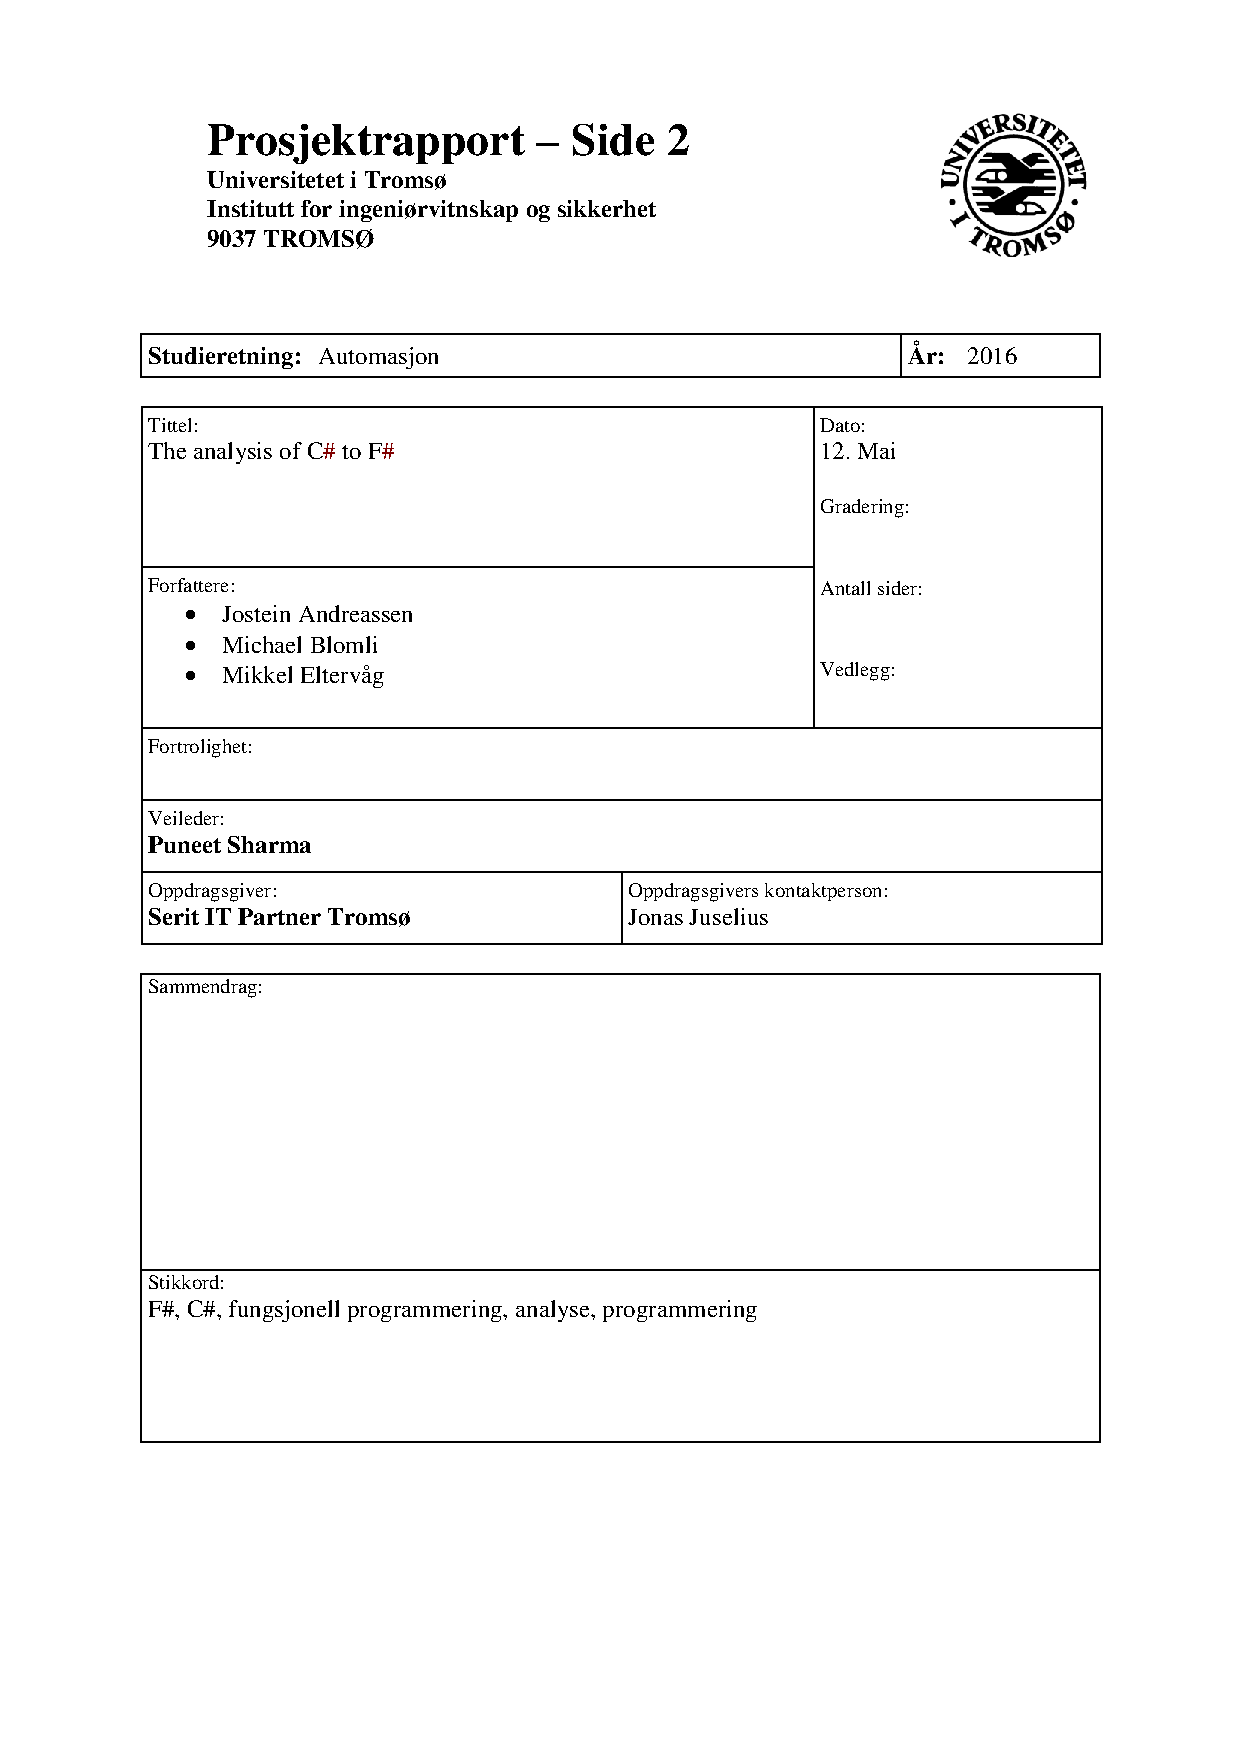
\includepdf[pages=-]{page2.pdf}
\newpage


\makebox{\vbox to 0pt{\hfill
\makebox{
\includegraphics[height=2.5cm]{LogoEngelsk}}}}

\textbf{\Large Project rapport - Page 2}\\

\textbf{Universitetet i Tromsø}\\
\textbf{Institutt for ingeniørvitenskap og sikkerhet}\\
\textbf{9037 TROMSØ}\\

\begin{tabularx}{\textwidth}{|p{9cm}|X|}
 	\hline
 	\pbox{\textwidth}{
 		\vspace{1mm}
 		\textbf{Study:} Automation
	} 
 	&
 	\pbox{\textwidth}{
 		\vspace{1mm}
 		\textbf{Year:} 2016
	}
	\\
 \hline
\end{tabularx}\\

\begin{tabularx}{\textwidth}{|p{9cm}|X|}
 	
 	\hline
 	\parbox[t]{\textwidth}{
 		\vspace{1mm}
 		\textbf{Title:}\\
 		The analysis of C\# to F\#\\[2mm]
 		\textbf{Authors:}\\
 		Jostein Andreassen\\
 		Michael Blomli\\
 		Mikkel Eltervåg
 		
	}
 	
 	&
 	\parbox[t]{\textwidth}{
 		\vspace{1mm}
 		\textbf{Date:}\\
 		May 12th\\[2mm]
 		\textbf{Classification:}\\ 
 		Open\\[2mm]
 		\textbf{Pages:}\\
 		\pageref{LastPage} \\[2mm]
 		\textbf{Attachments:}\\
 		4\\
	}
 	\\
 	\hline
\end{tabularx}

\begin{tabularx}{\textwidth}{|X|}
\pbox{\textwidth}{
\vspace{1mm}
\textbf{Mentor:}\\
Puneet Sharma
\vspace{1mm}
}
\\
\hline
\end{tabularx}

\begin{tabularx}{\textwidth}{|X|X|}
 	\pbox{\textwidth}{
 		\vspace{1mm}
 		\textbf{Contracting entity:}\\
 		Serit IT Partner Tromsø
 		\vspace{1mm}
	} 
 	&
 	\pbox{\textwidth}{
 		\vspace{1mm}
 		\textbf{Contact person:}\\
 		Jonas Juselius
 		\vspace{1mm}
	}
	\\
 \hline
\end{tabularx}\\[3mm]



\begin{tabularx}{\textwidth}{|X|}
\hline
\pbox{\linewidth}{
\vspace{1mm}
\textbf{Summary:}\\
In this report do we an analysis of a new programming language called F\#. This analysis is written for Serit IT Partner  to look at the possibility that F\# can be a replacement for the programming language they are using today that is C\#.\\[2mm]
To help us write this analysis we have translated and optimized a program that Serit have written. This is to get an understanding of the benefits and drawbacks of changing from C\# to F\#. We have also looked at code examples that others have written and looked at what experiences that company's that already have changed language has.\\[2mm]
Our conlution is that F\# should not completely replace C\# as their main programming language. F\# should be used together with C\# to get the benefits of both languages. 
\vspace{1mm}
}
\\
\hline
\pbox{\linewidth}{
\vspace{1mm}
\textbf{Keywords:}\\
F\#, C\#, Functional programming, analysis, programming, SQL
\vspace{1mm}
}
\\

\hline
\end{tabularx}


\newpage
\section*{Summary}
This report is written by 3 students from the final year in the Automation class at “UiT: University of Tromsø - Arctic university of Norway”.\\

The assignment is given by a company named Serit IT Partner from Tromsø. They wanted us to identify the benefits, flaws and our experience from learning a new programming language called F\#. Today Serit mostly uses the famous programming language C\# which is currently widely used around the world. The time spent writing code and debugging, and the stability in these languages is very valuable. Serit IT Partner wanted us to test out if a change of main programming language from C\# to F\# would have an impact on time spent on coding, reduce the number of lines of code and would improve stability.\\

We found that we could clearly see a difference regarding the numbers of lines of code and the performance in the application that was given to us. Indeed, F\# is better (or perhaps, more convenient) than C\# in some cases. F\# is a programming language which is very good at handling large amounts of data, and is also good with concurrency (dealing with multiple things at the same time). Due to the nature of the language, large operations on data can be broken down into smaller tasks and calculations can be made without fear of unintended side effects.\\

We started out at thinking that F\# was out there to replace C\#, however that was not the case. F\# is made as a tool that should work together with C\# seamlessly to make great applications. Both programs are used in the .NET framework and by that they work very well together. F\# doesn't need to completely replace C\#, instead it should be implemented there where it is suited best. Based on our results Serit should consider starting a small team and use F\# where it’s best and easy to implement and use C\# where its better. Then they could gradually expand the F\# team if they see the need for it.

\newpage
\section*{Preface}
This thesis is written by graduates from the automation program at the department of engineering  at UiT: University of Tromsø - The Arctic University of Norway. This thesis will be used by Serit to help them determine whether incorporating the F\# programming language would be favourable for the company.\\

We chose this assignment because everyone in our group enjoys programming, the assignment had some database management and set up, and because it looked like an interesting project overall. Since we already had some experience in C\#, we thought it would be fun to find the “pros and cons” of this relatively new programming language.\\

We have written the thesis in LaTeX which is a word processor and a document markup language. When we were working on the raw text we used Google documents so that we all could work together simultaneously on writing and editing the text for the thesis. On the main assignment we used Visual Studio (with C\# and F\# tools), Atlassian Sourcetree and Github to write and manage our code, and SQL Server Management Studio to handle the database. By using both C\# and database we covered a wide area of our syllabus from the previous semester. We have learnt a lot and have had the privilege of testing out the new attractive programming language F\# that may just be the future. \\

We want to give out a special thanks to Jonas Juselius and Jens Blomli at Serit for all the great support and advice given, on all the regular follow up meetings and by email. We also want to give a big thanks to our mentor Puneet Sharma for his great support and contribution to the assignment.\\

\newpage
\tableofcontents

\newpage
\section{Introduction}
\subsection{Background}
One of the biggest problems in modern application development is the rapidly growing complexity of all major software systems. This complexity makes it almost impossible to ensure quality and accuracy of the code. It also becomes harder and harder to make changes to existing code without introducing new errors. All these difficulties multiply when one attempts to utilize modern computers with many CPU (central processing unit) cores for increased performance.\\

The imperative object-oriented programming paradigm has been dominant in software development for over 20 years. In the imperative paradigm the state variables will be handled explicitly, which can quickly give too much complexity. The functional programming paradigm has been known since the 1930’s, but has not been popular with professional developers because of the slightly lower (single core) performance and greater resource use. Today these obstacles are long gone, and functional programming is experiencing a new renaissance due to significantly better control over complexity and parallelism.\\

%We've received an assignment from Serit to translate parts of an existing project from C\# code to F\# code.
C\# is meant to be a simple, modern, flexible and object oriented programming language. It is developed and maintained by Microsoft and is inspired by previous popular object-oriented languages like C++ and Java. F\# is a hybrid language that supports both the familiar object-oriented method and functional programming. F\# is also developed by Microsoft, and like C\# also has access to Microsoft’s .NET framework. 
%Serit wants us to find out the benefits of  switching from the programming language C\# development to F\#.\\

\newpage
\subsection{Problem for discussion}
Programming in C\# and F\# works in different ways, they both have benefits and drawbacks. The main question is whether it is worth it for a company to change their main programming language, in other words if the benefits outweigh the drawbacks of implementing this new language. We have to look at what the company wants to achieve by making the change, and that boils down to making quality programs for a low price. \\

A modern IT company uses a lot of time developing, changing and fixing code. If we can use a programming language that takes less time to develop and at the same time works better without generating errors, cost saving could be achieved.\\

The programming language F\# claims to be a solution to these problems by using fewer lines of code, be more simple to write, be easier to understand and have better error handling than other programming languages. Our task is to uncover whether those claims are true by answering the following questions:

\begin{itemize}
\item What are the benefits of switching from C\# to F\#?
\item To what degree can we reduce the number of lines written in the program code?
\item How much time is saved in the debugging stage?
\item How much time is saved in the development of the code?
\end{itemize}

\newpage

\subsection{Formulations of objectives}
%To work on an analysis (compare code) of the old code compared to the new code, where we will look at how compact the code is, how many errors there are, how self-explaining the code is and how easy it is to develop the code.

Serit IT Partner want to find out if it is worth changing their main programming language from C\# to F\#. Our task is to do an analysis and make our own conclusion to help them make their decision. This is achieved by reaching the objectives presented below.

\begin{itemize}

	\item Learn to program in F\# to:
	\begin{itemize}
		\item get a good enough understanding of how to write simple programs.
		\item see how it is for a programmer to learn the new language.
		\item get our own opinions about the language.
	\end{itemize}
	
	\item Learn from translating a real program from Serit by:
	\begin{itemize}
		\item finding the best translation method.
		\item looking at the development process for F\#.
		\item learning how F\# handles the databases.
		\item looking at how F\# deals with debugging and error handling.
		
	\end{itemize}
	\item Learn from online research by looking at:
	\begin{itemize}
		\item other people's opinions about F\#.
		\item how other companies take advantage of F\#.
		\item good code examples that others have written.
		\item what are some good usages of F\#.
	\end{itemize}
	
	\item Write a complete analysis that contains information about:
	\begin{itemize}
		\item development time.
		\item readability and clarity.
		\item debugging and error handling.
		\item performance.
		\item our experiences.
	\end{itemize}
	
	\item Draw a conclusion to consider whether it is valuable for Serit to change their main programming language from C\# to F\#.
	
\end{itemize}


\newpage

\subsection{Different programming paradigms}
There are many different ways of classifying programming languages and styles. One of the most common ways of classifying is imperative versus declarative programming. The distinction is that imperative programming states the order in which the operations execute, while declarative does not. Another important feature is if side effects are allowed or not. By this, we mean if a function or subroutine can change the state of other parts of the program. In imperative programming, this is allowed, while in functional programming, it is not. Finally, there are different ways of organizing programs and breaking down problems into smaller, reusable pieces. Procedural programming focuses on breaking down the program into functions (also commonly called subroutines). Object-oriented programming organizes the program by grouping together the functions (methods) with the state they are allowed to modify (properties).

\paragraph{Imperative} Imperative programming is a paradigm where statements are used to tell the computer program what to do. It is the programmer’s job to tell the computer how to solve the problem. If an imperative program were to make a person get a cup of coffee, it would have to list all the individual tasks they had to do, like stand up, walk to the coffee machine, place the cup, press the button and so on. 

\paragraph{Declarative} Declarative programming focuses instead on telling the computer program what the desired result is, and then the implementation of the programming language decides how to do it. A declarative program would simply state “Give me a cup of espresso”. Examples of declarative programming include database query languages and functional programming.

\paragraph{Functional} Functional programming is a form of declarative programming. Instead of using statements, like in imperative programming, functional programming uses expressions. An expression is a combination of one or more values, operators or functions that produce a resulting value when evaluated. A goal in functional programming is to limit side effects and mutable values. This means that if you call a function with the same arguments you should get the same result everytime. Thus, the output of a function should only rely on the inputs to that function, and not any other values or variables.

\newpage
\paragraph{Procedural} Procedural programming breaks programs down into subroutines or functions which take arguments as input, and produces an output or result that is sent back to the caller. Functions can be designed to be as generic as possible so they can be used again in many parts of the program, which means less repetition of code.

\paragraph{Object-oriented} On the other hand, Object-oriented programming focuses on categorizing the entities in the program as different objects, that expose behavior and data using interfaces. Objects may contain both data and methods. Methods are functions that are only allowed to change the data of the object to which it belongs. This is a way of protecting against side effects that is called encapsulation.


\newpage
\subsection{F\# programming language}
F\# is a modern multi-paradigm programming language with a focus on functional programming. It was originally invented as an implementation of the OCaml language (which comes from ML) in the .NET platform. The first stable version was F\# 2.0 which came in 2010. F\# is open source and cross platform. F\# was influenced by a number of other languages. It gets it’s object model from C\#. Sequence expressions and computation expressions come from Haskell. Finally, the indentation-aware syntax was inspired by Python. F\# began as a .NET language, working together with C\# and .NET libraries. It can also be compiled to Android, Apple iOS, Linux, JavaScript, and GPU code.\\

F\# is “functional first” which means that functional programming is the preferred go-to method for solving problems. However, unlike many other functional languages, F\# works well with imperative and object-oriented programming where those styles are required. F\# is statically typed and type-safe which means the compiler can optimize the code deeply to increase performance, which is not possible in dynamic languages where types do not need to be known during compilation. Despite this, since F\# uses type inference (the compiler deduces what type a value has based on the context and data) it can be more expressive, like a dynamic language.\\

There are four main differences between F\# and a standard imperative language such as C\# or Java.
\begin{itemize}
\item Function-oriented rather than object-oriented
\item Expressions rather than statements
\item Algebraic types for creating domain models
\item Pattern matching for control flow
\end{itemize}

\paragraph{Function oriented}
In F\#, functions are First-Class Citizens. This means that functions can be passed as arguments, returned from functions, and assigned to values. Composition is the technique of making basic functions, then functions that use those functions, and so on. Functional code is by it’s nature high level and declarative.

\paragraph{Expressions}
In functional languages, there are no statements, only expression. Every code chunk must always return a value. Rather than using a list of statements that are executed in order, larger chunks of code are created by combining smaller chunks. There are no such thing as unassigned values, they must be assigned to when declared. Every possible branch of a control flow construct must be explicitly handled and must also return the same type. This makes code built from expressions safer than code using statements.

\paragraph{Algebraic types}
In F\#, new compound types are built by combining existing types in two different ways. First, a combination of values from a set of types. These are called product types, and are similar to structs or record types from other languages. Second, a disjoint union, representing a choice of types. These are called sum types.

\paragraph{Pattern matching}
Imperative languages have many different constructs for control flow and looping, including if-then-else, switch and case, for, foreach and while. In F\#, all of these can be replaced by pattern matching and the single keyword match. Conditionals such as if and switch are replaced by simple pattern matching, and loops are replaced by pattern matching and recursion. And finally, inheritance, a defining feature of object-oriented programming can be replaced by pattern matching on union types.

\begin{shadequote}{From the foreword of the book Expert F\#}
F\# is unique amongst both imperative and declarative languages in that it is the golden middle road where these two extremes converge. F\# takes the best features of both paradigms and tastefully combines them in a highly productive and elegant language that both scientists and developers identify with. F\# makes programmers better mathematicians and mathematicians better programmers.
\end{shadequote}



\newpage
\subsection{Project specification }

\subsubsection{Where Serit is now}

\begin{itemize}
	\item They have an ASP.NET Web application in C\# where the user interface is based on ASP Web Forms. All code is written in English, as well as all the text in the user interface.
	\item Language support is dissolved in a separate library sCore.Translation which is called from the application and performs translation according to data recorded in a translation table.
	\item Translation tables are located in a SQL database.

\end{itemize}

\begin{figure}[!h]
    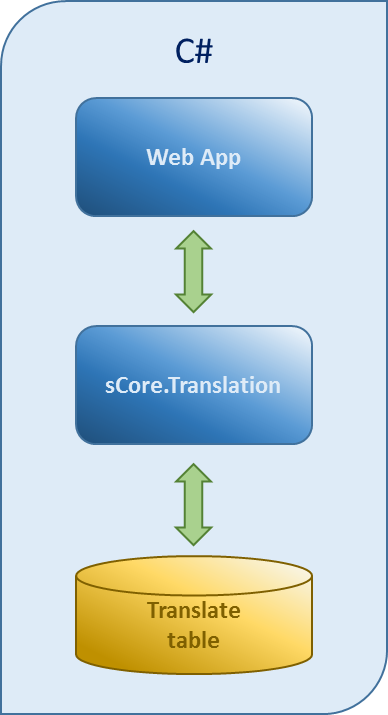
\includegraphics[scale=0.4]{image00}
    \centering
    \caption{How the communication of Serit's sCore.Translation application looks now.}
\end{figure}

\newpage
\subsubsection{What Serit wants}

\begin{itemize}
	\item They want to have the existing translation library sCore.Translation developed as a separate library in the functional language F\#. This should be able to be called from the present imperative program (C\#) and from functional programs (F\#).
	\item With the translation from C\# to F\# done, both languages and programming paradigms can be compared analytically. By this we can evaluate benefits (and possible disadvantages) with the functional paradigm in relation to an object-oriented imperative paradigm. The analysis will provide a better basis in the choice of programming language in future development projects.
\end{itemize}

\begin{figure}[!h]
    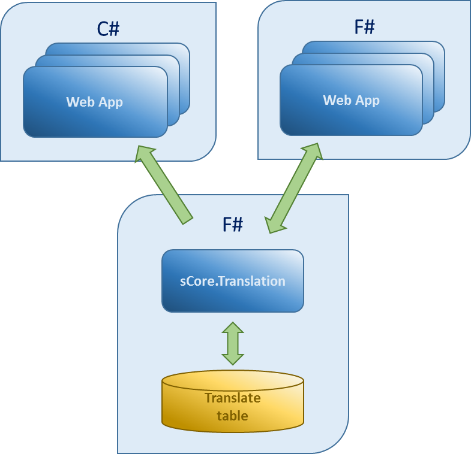
\includegraphics[scale=0.5]{image02}
    \centering
    \caption{How they want the sCore.Translation application to communicate.}
\end{figure}

\newpage
\subsubsection{Method of translation}
F\# for fun and profit describes three levels of “sophistication” for porting code from C\# to F\#. The basic level is simply a direct port. Since F\# supports imperative programming, it can be translated directly. At the intermediate level, the code is refactored to be fully functional. The advanced level takes advantage of F\#’s data type system.\\

There are two paths to achieve this goal: Either by first porting to F\# and then refactoring to functional code, or by converting to functional code in C\# before porting that to F\#.

\begin{figure}[!h]
    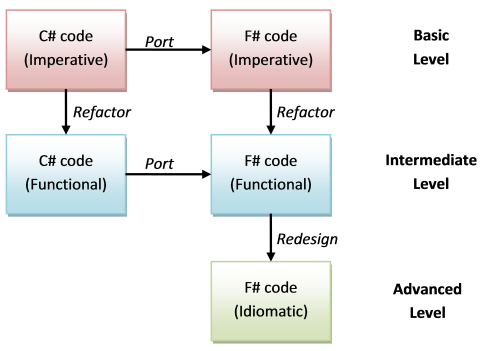
\includegraphics[scale=0.6]{image01}
    \centering
    \caption{Method's of translating from C\# to F\#.}
\end{figure}



\newpage

\section{sTranslate}
sTranslate is a library that is part of a bigger program. The purpose of the library is to take a phrase and some meta-data as arguments (inputs) and then use a language database to translate the phrase (output).\\

The library is written in C\# and contains two major functions, one is designed to use when you are only going to translate one word or phrase, and the other one is designed to be better (faster) at doing multiple translations in succession. Even though the function works differently they have the same inputs and outputs, that means that they do the same thing if you look at it from the outside. You can see an illustration of the library in figure \ref{fig:sTranslateWorkings}.\\


Our task from Serit is to take this C\# code and translate it into F\# with two different approaches. The first one we translate line for line and program in an imperative style, the same way that the C\# program is coded. The other one is to refactor the program to a more functional approach, the way F\# is meant to be written. After we have translated it we have to do look at how we can optimize the code to improve performance and readability while reducing the number of lines of code. Finally we will compare and analyze it against C\# and look at performance, difficulty of programming and all other obvious differences.\\

\begin{figure}[!h]
    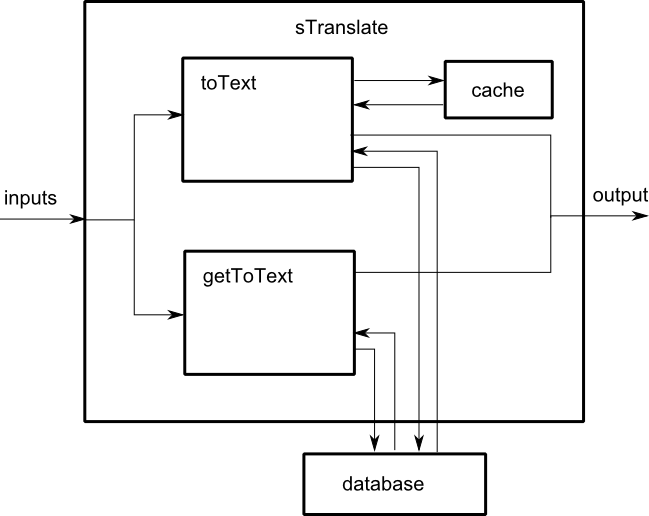
\includegraphics[width=0.8\textwidth]{sTranslateWorkings}
    \centering
    \caption{sTranslate library illustrated.}
    \label{fig:sTranslateWorkings}
\end{figure}

\newpage
\subsection{How it works}
The sTranslate library is supposed to be used with both C\# and F\# programs. It is important that the library takes the same inputs and outputs in both languages. Figure \ref{fig:sTranslate_communication} show this communication.

\begin{figure}[!h]
    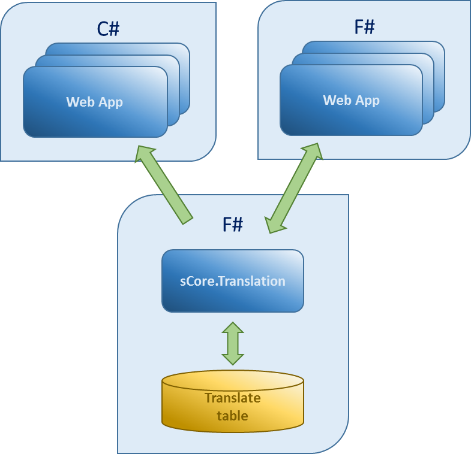
\includegraphics[scale=0.5]{image02}
    \centering
    \caption{How Serit want the sCore.Translation application to communicate.}
    \label{fig:sTranslate_communication}
\end{figure}

The main part of the library is the following functions: toText and getToText, as shown in figure \ref{fig:sTranslateWorkings}. Both functions do the same thing but there are one major difference between them. In getToText you have to open the language database each time you want a translation, but in toText the database is cached (stored in program memory) so it does not need to reopen the database for each search.\\

\newpage
\subsubsection{Inputs and Outputs}
The sTranslate library should in theory work well for a pure functional approach. The output of the functions should only depend on the input, which will be the phrase to translate, it's metadata, and the contents of the database itself (which we can assume to no change while the search is happening).\\

A key part of the viability of F\# will be to see how easy it is to compile a library that is compatible with C\# programs. This should be trivial due to the close integration with the .NET system. A C\# program should easily give inputs or take outputs from F\# and the other way around. How we are going to use this feature can be seen in figure \ref{fig:sTranslate_communication}.\\

sTranslate is taking in 5 inputs:

\begin{itemize}
	\item \textbf{fromText}, the phrase in English that the library is translating. 
	\item \textbf{context}, information over how the phrase is used, examples: string, title, lable.  
	\item \textbf{property}, category information about the phrase, examples: id, text, tooltlip...  
	\item \textbf{criteria}, position of the phrase in a sentence, examples: startWith, endWith, Contains.
	\item \textbf{toLang}, the target language of the translation, examples: no, ge.
\end{itemize}

sTranslate gives only one output, which is the translated phrase (a string). All the inputs have to match up to the row in the database to send the output. In there is no match, fromText (the English phrase) will be sent back as output and if the search algorithm finds duplicate rows (multiple matches), only the first one will be selected.\\


\newpage

\subsection{Solution}
When porting code from C\# to F\# there are two ways of refactoring the code into being functional. The first is to translate the C\# code directly to F\#, almost line by line, and then refactor the F\# imperative code into functional code. The second way is to use the functional programming tools in C\# to refactor the program, and then translating that to F\#. We chose to use the first method.\\

In the figures below, we show an extremely simple code example of translating a piece of C\# code to F\# using an iterative approach. First the code is translated directly, then the \code{if-then-else} construct is replaced by pattern matching to make it more functional. It is important to remember that for such a simple code, the \code{if} construct would actually work fine in F\# (see figure \ref{fig:directTranslationIf}). This is because \code{if} constructs work a little different in F\#: The entire if is itself an expression, and both (or all) conditional branches must evaluate to the same type. In this case, writing to the console evaluates to \code{unit()}. Since both branches evaluate to \code{unit()}, the expression is valid. Similarly, when using pattern matching for control flow as in figure \ref{fig:functionalApproachIf}, all patterns must evaluate to the same type, and just like \code{Console.WriteLine}, the \code{printfn} function evaluates to \code{unit()}.\\

For a complete study of the different versions of the sTranslate program, the complete libraries with comments are documented in attachments (insert ref later). In this chapter, we will first be taking a closer look at one part of the program, which is the part that reads the database and provides a list that another function can use to perform the search. Then we will examine some parts of the final F\# program and see how and why it differs from the C\# program. Finally, we tried to go even further beyond, and made a version of the program that, while it doesn't quite interface with Serit's web application, does show off some of the power and elegance of the F\# language. This version of the library uses high performance data structures and parallel programming to translate a large number of queries very quickly.

\newpage

\subsubsection{Basic code examples}
In the figures below are shown code chunks with identical functionality, one written in C\# and two different ways of doing it in F\#.

\begin{figure}[!h]
\begin{lstlisting}
if (a == b){
	Console.WriteLine("equal");
}
else{
	Console.WriteLine("not equal");
}
\end{lstlisting}
\caption{C\# code example}
\label{fig:CSharpIf}
\end{figure}

\begin{figure}[!h]
\begin{lstlisting}
if a = b then 
	Console.WriteLine("equal")
else 
	Console.WriteLine("not equal")
\end{lstlisting}
\caption{Direct translation code example}
\label{fig:directTranslationIf}
\end{figure}

\begin{figure}[!h]
\begin{lstlisting}
match a with
    | b when a = b -> printfn "equal"
    | _ -> printfn "not equal"
\end{lstlisting}
\caption{Functional approach code example}
\label{fig:functionalApproachIf}
\end{figure}

\newpage


\subsubsection{The GetTranslations function in 3 different ways}
\paragraph{C\# version from Serit} A private variable is declared whose purpose it is to hold the contents of the database when the user calls the \code{toText} function. This variable is visible to all functions inside the \code{XltTool} class, but not to external users of the class. The \code{GetTranslations} function both mutates the \code{\_translateColl} variable, and has it as a return value. Since the function is public, this makes the contents of \code{\_translateColl} accessible to users. The \code{GetTranslations} function will open and read the database if either the \code{\_translateColl} variable is empty, or the user has specified that it wants to read the database again.

\begin{figure}[!h]
\begin{lstlisting}
private static List<Model.Translation> _translateColl = null; 
public static List<Model.Translation> GetTranslations(bool reRead = false)
{
    if (_translateColl == null || reRead == true)
    {
        using (var ctx = new Model.TranslationEntities())
        {
            _translateColl = (from xl in ctx.Translation select xl).ToList();
            if (_translateColl == null)
                _translateColl = new List<Model.Translation>();
            return _translateColl;
        }
    }
    return _translateColl;
}
\end{lstlisting}
\caption{C\# version of the GetTranslations function}
\end{figure}

\newpage


\paragraph{F\# Imperative version} The imperative version retained the functionality of the C\# version. The function is called and makes changes to a mutable value, and also returns that value to the caller. Note that we are still using mutable values even if we are working with F\#.

\begin{figure}[!h]
\begin{lstlisting}
let mutable _translateColl : List<Translation> = []
let GetTranslations (reRead : bool) =
    if _translateColl = [] || reRead = true then
        use db = dbSchema.GetDataContext(Settings.ConnectionStrings.DbConnectionString)
        _translateColl <- 
        query {
            for xl in db.Translation do 
                select xl
        } |> Seq.toList |> List.map toTranslation
\end{lstlisting}
\caption{Direct translation of the code}
\end{figure}

\newpage


\paragraph{F\# Functional version} The functional version gets rid of the mutable value alltogether. The \code{GetTranslations} function uses the \code{FSharp.Data.TypeProviders} library, which gives typed access to the tables of the database. The Type Provider handles caching of the database automatically, so we can get rid of the “storage variable” that was used in the imperative version. The \code{GetTranslations} expression is evaluated once when it is needed, and then the data is there, ready to be used until the program ends.

\begin{figure}[!h]
\begin{lstlisting}
let GetTranslations =
    use db = dbSchema.GetDataContext(Settings.ConnectionStrings.DbConnectionString)
    query {
        for row in db.Translation do 
            select row
    } |> Seq.toList |> List.map toTranslation 
\end{lstlisting}
\caption{Refactored to functional code}
\end{figure}

\newpage


\subsubsection{Detailed look at F\# sTranslate}
There are a few key points where the functional F\# library differs from the C\# version:
\begin{itemize}
	\item The F\# SQL Type Provider is used instead of EntityFramework.
	\item GetToText takes Option string arguments instead of Enums.
	\item GetTranslations produces an immutable list.
	\item The ToText function was removed as it was obsolete.
\end{itemize}

\paragraph{F\# SQL Type Provider} 

\paragraph{Option type arguments}

\paragraph{Getting the database}

\paragraph{Removal of obsolete function}


\newpage


\subsubsection{Parallel version of sTranslate}

\newpage


\subsection{Analysis}
In this chapter we will take a look at the analysis of the module sTranslate.
Looking back on how we used the two different methods of writing the F\# code, the line by line translation and the functional approach, we can say that the direct translation was clearly not the way to go. It became much harder to do the actual programming in an object-oriented way, so much that we even ended up doing the direct translation without using classes at all (while the C\# code of course did have classes). We found that by using the direct translation, we didn't really save many lines of code. We could also notice in the result a clear difference in the actual speed of the program, where the direct translation was inferior to the functional code. We get into this a little more later.

\subsubsection{Performance}
This chapter is not a demand from Serit, instead this was something we wanted to test out for ourselves, and is just a bonus for Serit if it proves to be better performance in F\# vs C\#.
\subsubsection{Experiences}
The experiences that we can draw from this assignment is that in F\#, it’s very easy to read the code and what it does, and that you almost don’t need to comment the code. But the thing we appreciated the most was the direct response from the compiler and Microsoft’s Intellisense technology in real time while writing the code. At first we thought that this was a bit unfavourable since you always saw errors made in code with the red lines everywhere. However, as the language is very strict about types and such, one is forced to root out many errors before the program even is able to run. Because programming with pure functions eleminates side effects and state changes, the programmer won't have to deal with unexpected errors later while running the program, which could make it misbehave or even crash. Hence we grew to really enjoy this feature. It makes the programmer put a little more time in thinking about what they want the code to do, but they will spend less time dealing with problems later.\\

Since all the group members have object-oriented programming background, the main struggle we experienced was our tendency to get back to old habits and thinking in the object-oriented way of programming. The new thinking in functional programming was harder than we imagined. We acknowlegded that it’s probably easier for a person who have never done programming before to learn F\# then a person coming from a background with object-oriented programming at least in some aspects. Of course, that is not completely true because a skilled programmer can quickly find patterns in the code and structure, this varies from programmer to programmer. We had to let go of a lot of hard learned coding and try and think “out of the box” to be able to write “decent” F\# code.\\

We realised that everytime we went ack to the written code, improvements could be made both in terms of code length but also with regards to quality. F\# is mainly a function based programming but it actually allows imperative and object-oriented programming in some way. Since it’s integrated into Visual Studio and the .NET framework there are a lot of features inherited from C\#. That will allow the user to use for loops, if-else constructs, mutable values, etc. Still, we found that all of these thing were replacable when programming functionally.\\

For Michael, the biggest struggle of this experience was that he kept finding himself getting back in think in object-oriented “thinking”. It's hard to think in a more functional approach.\\
\subsubsection{Lines of code}
When it breaks down to how many lines of code there is in each project we can right away see big differences.\\

Here is a short outline on how many files and lines each project got:\\

\begin{tabular}{ |p{4cm}|p{3cm}|p{2cm}|p{3cm}|  }
 \hline
 \multicolumn{4}{|c|}{Short outline} \\
 \hline
 Language & Lines of code & Files & Projects\\
 \hline
 C\# & 280 & 3 & 2\\
 F\# imperative style & 170 & 4 & 1\\
 F\# functional style & 145 & 2 & 1\\
 \hline
\end{tabular}

\newpage

\section{Online research}

\newpage
\subsection{Testimonials}

To get a better understanding of how companies could benefit using F\# do we have to look at what experiences programmers and companies have with F\#. The internet contains a lot of testimonials where people write their personal experiences with F\#. It is important to note that those companies have already done the choice of using F\# in their applications. This means that they have found F\# useful and therefore more likely to talk possessively about the language. Here we have taken some of those testimonials to take a closer look.

\paragraph{Simon Cousins}

Simon is a developer at UK-based Power Company. He uses both C\# and F\# to write his applications. What we can learn from what he have written is that F\# and C\# can be used together. He uses C\# to write the client and server components and F\# to write the calculation engine. This is a really smart usage of both programming languages as he uses the best language to each task.\\

He does also write that he is still waiting for the first bug from a bug to came in from a delivered F\# project and that this is not the case with C\#. Here we can see the effect of the strong type system in the F\# compiler.

\begin{shadequote}{Simon Cousins}
I have now delivered three business critical projects written in F\#. I am still waiting for the first bug to come in.
\end{shadequote}

\paragraph{Michael Newton}

Michael is a Senior Developer at a development company named 15below. Historically they have written their code in a mix of C\# and VB.NET. They uses F\# for components where the language strength's shine, without discarding or rewrite the existing code.\\

What we can learn from this is that is really well integrated with the .NET framework. This makes it really easy to use with the code that the company already have written. That can be really beneficial for Serit IT Partner as their code today is written in C\# that supports .NET. 

\begin{shadequote}{Michael Newton}
We would recommend F\# as an additional tool in the kit of any company building software on the .NET stack.
\end{shadequote}

%\newpage

%\paragraph{Marty Dill}

%\begin{shadequote}{Marty Dill}
%\end{shadequote}


%\paragraph{}

%\begin{shadequote}{}
%\end{shadequote}

\newpage
\subsection{Code examples}
We have done some research on the web to find some concrete code examples to highlight some differences in these two coding languages.

\subsubsection{Basic from 1 to N square function}
\paragraph{F\#}
A lot of our research comes from the web page fsharpforfunandprofit, and there they highlight a simple task where they sum the squares from 1 to N. We can see how the code could look like if it was written in F\# in figure \ref{fig:SquareFunctionFSharp}.

\begin{figure}[!h]
\begin{lstlisting}
// define the square function
let square x = x * x

// define the sumOfSquares function
let sumOfSquares n = 
   [1..n] |> List.map square |> List.sum
\end{lstlisting}
\caption{Basic from 1 to N square function made in F\#.}
\label{fig:SquareFunctionFSharp}
\end{figure}

Here they made 2 functions, where one uses the other function as an output on it’s own. The \code{|>} is used to send the output from one function and send it as an input to the other.
If we break this down to what it does it’s basically, first an function is made that is called square, it simply takes itself and multiply it with itself. Then an other function is made sumOfSquares, it makes a loop from 1 to n, then puts them into a list and each element is used with the square function. Then it sums the list up and sends it back as the output. We didn’t need to do any type declarations, because the compiler figured out that it has to be an integer. That is because the input in sumOfSquares is used to create an array, and that needs an integer. If we now try to write a piece of code that would send for example a floating point number to that function, the program wouldn’t even compile, and you would save yourself some debugging time.\\

\newpage

\paragraph{C\#}
Now if we take a look at how the code would look like in classic C\# (non-functional) style of a C-based language. First we take a look at the code seen in figure \ref{fig:SquareFunctionCSharp} below.

\begin{figure}[!h]
\begin{lstlisting}
public static class SumOfSquaresHelper
{
   public static int Square(int i)
   {
      return i * i;
   }

   public static int SumOfSquares(int n)
   {
      int sum = 0;
      for (int i = 1; i <= n; i++)
      {
         sum += Square(i);
      }
      return sum;
   }
}
\end{lstlisting}
\caption{Basic from 1 to N square function made in C\#.}
\label{fig:SquareFunctionCSharp}
\end{figure}

So this code basically does the same thing. The interesting part here is that what F\# could to with 2-3 lines of code, the basic C\# would to in about 16 (to be fair most of the lines is just { and }) that is pretty impressive. However you could make this much more compact but that would make it much harder to read, since this is the standard that is mostly used.\\

So to highlight the differences of these two code examples. First it is that the F\# code is much more compact and still is very readable (almost self explained). The F\# code didn't have any type declarations (f.ex C\# have to do int sum = 0, before sum is even used). The last thing is that F\# can be developed interactively. With that we mean that we can test the functions right away and check if we get back what we want or not without having to go in and out of functions with the use on the interactive window that F\# has.

\newpage

\paragraph{C\# LINQ}
Today many C\# programmers uses LINQ, a much more modern tool with C\# that in someway lets C\# be more functional.\\

So let’s take a look at how the code would look like using the C\# LINQ extension, we can see this in figure \ref{fig:SquareFunctionCSharpLINQ} below.

\begin{figure}[!h]
\begin{lstlisting}
public static class FunctionalSumOfSquaresHelper
{
   public static int SumOfSquares(int n)
   {
      return Enumerable.Range(1, n)
         .Select(i => i * i)
         .Sum();
   }
}
\end{lstlisting}
\caption{Basic from 1 to N square function made in C\# LINQ.}
\label{fig:SquareFunctionCSharpLINQ}
\end{figure}

We took the basic C\# code from 16 lines down to 9 lines. This almost took down the C\# code to half, but still not near the F\# code. Also here we can see that the C\# code is bound to use the  curly braces and periods and semicolons. The code also still needs to be declared to be able to use variables, that we don’t need to do in F\#.

What we can conclude with this short example is that F\# in this case was superior in many ways, more easy to read, more compact and you can easily check the gained outputs through the interactive window. 

\newpage
\subsection{Rotate a tuple}
Here we are gonna take a look at one more example, this time very short and easy function. The function simply is used to change the order of a tuple (a tuple is set of values, f.ex. cordinates in an aksis).\\
   
\paragraph{F\#}
First lets take a look on how we would to this in F\#, we can se this in figure below.

\begin{figure}[!h]
\begin{lstlisting}
let rotate (x,y,z) = (z,x,y)
\end{lstlisting}
\caption{Rotate a tuple example made in F\#}
\label{fig:RotateTupleFSharp}
\end{figure}

\paragraph{C\#}
Since we can’t just rearrange the order easily on a tuple in C\#, we have to do it in a little different approach. This is shown in figure below.\\

\begin{figure}[!h]
\begin{lstlisting}
Tuple<V,T,U> Rotate(Tuple<T,U,V> t) 
{ 
    return new Tuple<V,T,U>(t.Item3,t.Item1,t.Item2); 
}
\end{lstlisting}
\caption{Rotate a tuple example made in C\#}
\label{fig:RotateTupleCSharp}
\end{figure}

So firstly here we have to define that its a tuple first, and then give it a name and in this case it’s Rotate. When we are returning the new values we have to tell the compiler what tuple we are gonna return as well as ref to each item in the new tuple.\\

This is a good example to show how easy things can be done in F\#.

\newpage
\section{Complete analysis}
In this chapter we will take a look at the complete analysis of the previous chapters. 

\subsection{F\# compared to C\#}

\subsection{Development time}

\newpage
\subsection{Readability and clarity}
Readability and clarity is really important when writing code. The reason for this is that it is much easier to find and remove bugs and add future content. If the programmer does not need to use a lot of time simply to understand what the code is supposed to do. Poorly written code can cause a programmer to spend a lot of time familiarizing themselves with the code before they can do changes to it.\\

For the most part it is up to the programmer to write readable and clear code, but the programming language can have a lot to do with helping the programmer in this matter.\\

%Some programming languages like for example Assembly can be seen as programming language that makes it hard for the programmer to writhe readable code. Other like for example Python make it really easy for the programmer.\\

So the question is how does F\# do in this matter? How difficult is it to write readable and clear code. How would a bad or new programmer's code look like? And how readable is a perfect written code?

\newpage
\subsubsection{Indentation and code structure}
\label{indentationAndCodeStructure}
F\# is a whitespace sensitive programming language, this means that indentation do have a meaning and will be read when you compile the code. When you are using indentation the compiler will read the indented lines as a code block that belonging to the code above. You can see this illustrated by code in figure \ref{fig:indentationExample}.

\begin{figure}[!h]
	\begin{lstlisting}
let f = 	// Line 2-5 belongs to this block
	let x = // Line 3 is the sub code of this line
		5+5	
	let y=1
  	x+y
let a = f+2	// On the same indentation as line 1, starting a new block
	\end{lstlisting}
	\caption{Example of how indentation works in F\#.}
	\label{fig:indentationExample}
\end{figure}

That means that to some extent the F\# language force the programmer to write code that have good structure in the code. This can make it easier to understand and read the code even if you don't know it beforehand.\\

For an inexperienced programmer this can be a little confusing at fist. But as this is a really good practice to learn early on it can help the inexperienced programmer write better code.\\

In indentation and code structure, F\# really does a good jobb when it comes down to readability and clarity.

\newpage
\subsubsection{File structure}

In most programming languages the file structure have nothing to do in how the program is compiled or run. F\# does this a little different, all the files have to be in a specific order to run the program correct.\\

Whenever you call a function you have to make sure that the function is written before the call in the code is made. And since all the files are read in order you have to make sure that if the function is in another file it has to be placed above the current file in the file structure.\\

The most common way to organize the files in a project is to have all the files in the same folder. This makes it more transparent and easy to order the code. This way of organization can work really well for small and medium sized projects, but for really big projects it may be better to organize in multiple folders.\\

A good practice when organising the files is to only have one module per file and make the functions inside correspond to the file name.\\

\newpage
\subsubsection{Similarity to other coding languages}

\paragraph{ML Programming Language}

Even though F\# has taken inspiration from a lot of different modern programming languages it still have a lot of roots to ML. This is a old and not that popular programming language. This makes the syntax very different to how syntaxes normally looks like today, and can make the syntax hard to read and write to any programmer that are not used to ML or other similar programming languages.\\

If we take a close look at figure \ref{fig:factorialMLExample} and \ref{fig:factorialFsharpExample} we see a lot of similarity in how the programs work. In the F\# example we can read match, that is a way of doing pattern matching. The ML code does also use pattern matching with a small change in the syntax. Line 1 in the ML code we can see that if the function gets a 0 as an input the output will be 1, the same thing happens at line 3 in the F\# example. Line 2 in the ML code tells us that if the input is an int the output will be \code{n * factorial (n-1)} and the same thing happens in F\# line 4 if the input is not 0.\\

\begin{figure}[!h]
	\begin{lstlisting}
fun factorial 0 = 1
  | factorial (n:int) = n * factorial (n-1)
	\end{lstlisting}
	\caption{ML code example of a recursion function (function that's call itself) that are calculating factorials. Example from Carnegie Mellon University\cite{carnegieMellon}}
	\label{fig:factorialMLExample}
\end{figure}

\begin{figure}[!h]
	\begin{lstlisting}
let rec factorial n =
    match n with
    | 0 -> 1
    | _ -> n * factorial (n - 1)
	\end{lstlisting}
	\caption{F\# code example of a recursion function (function that's call itself) that are calculating factorials.}
	\label{fig:factorialFsharpExample}
\end{figure}

\newpage
\paragraph{Python}

One programming language a lot of programmers can agree on being easy to read and understand is Python. Python is a language with a high level of abstraction, which means it acts as a "middle man" between the nitty gritty stuff that happens inside the computer, and abstract ideas. The syntax of Python has been designed to remove curly braces and semicolons that are used in languages like C and Java, using indentations instead to separate code blocks. Example of Python code can bee seen in figure \ref{fig:pythonFactorial}.\\

%\begin{figure}[!h]
%	\begin{lstlisting}
%print "Hello world!"
%	\end{lstlisting}
%	\caption{Hello world program in Python}
%	\label{fig:pythonHelloWorld}
%\end{figure}

\begin{figure}[!h]
	\begin{lstlisting}
def factorial(n):
    if n == 0:
        return 1
    else:
        return n * factorial(n-1)
	\end{lstlisting}
	\caption{Python code example of a recursive function (a function that calls itself) calculating factorials. Python also has a factorial function built in to the Math library. The equivalent F\# version of this program can be seen in figue \ref{fig:factorialFsharpExample}.}
	\label{fig:pythonFactorial}
\end{figure}

At a first glance Python and F\# can look similar because both languages is a white space sensitive programming language (Explained on page \ref{indentationAndCodeStructure}). But if you take a closer look at the programming languages they really works different, the main reason for this is that F\# is meant to be a functional programming language and Python is not, even though it have support for it.\\

Python is one of the programming languages that the creators of F\# have been using as a inspiration when making F\#. It is not hard to see the reason for this, because Python has an easy readability as an programming language. Both of them can be really self explanatory and forces the programmer to  write the code in a good structured way. This have made F\# more easy read and understand for programmers that looks at programs others have written.

\newpage
\paragraph{Assembly} One commonly used example for a programming language that is not easy to read or understand is Assembly. The reason that Assembly can be hard to read and understand for some people is that the programmer is working directly with CPU instructions and memory addressing. Even mundane tasks like moving a value to a registry must be explicitly programmed. In figure \ref{fig:assemblyExample} you can see an example of a "Hello world!" program. Most of the other programming languages does this in only one line . You can see an example of this in the F\# example in figure \ref{fig:fSharpHelloWorld}.\\

\begin{figure}[!h]
	\begin{lstlisting}
section	.text
    global _start   ;must be declared for linker (ld)
_start:	            ;tells linker entry point
    mov	edx,len     ;message length
    mov	ecx,msg     ;message to write
    mov	ebx,1       ;file descriptor (stdout)
    mov	eax,4       ;system call number (sys_write)
    int	0x80        ;call kernel
	
    mov	eax,1       ;system call number (sys_exit)
    int	0x80        ;call kernel

section	.data
msg db 'Hello, world!', 0xa  ;string to be printed
len equ $ - msg     ;length of the string
	\end{lstlisting}
	\caption{Assembly "Hello world!" code example from tutorialspoint.com \cite{tutorialspoint}.}
	\label{fig:assemblyExample}
\end{figure}

\begin{figure}[!h]
	\begin{lstlisting}
printfn "Hello, world!"
	\end{lstlisting}
	\caption{F\# "Hello world!" code example.}
	\label{fig:fSharpHelloWorld}
\end{figure}

It is maybe a little unfair to compare F\# with Assembly because Assembly is a really low level programming language. But there are two points that we can get out from this comparison and that is firstly that F\# is a easier language to write and understand, but this comes with the cost of less control over very basic computing that is important for really good optimization.

\newpage

%Old text below!

%\paragraph{F\# in comparison}

%One other thing that can make programming in F\#  when compared to other languages is that is it a functional programming language. This makes the syntax a lot different to all other major languages.\\

%Those two things makes F\# really different to other languages. This can make it very hard for a experienced programmer learning to read and write this way. For an experienced programmer to learn F\# you have to use a lot of time and resources. For a new programmer it can perhaps be easier to learn F\# just because they will not fall into old habits.

%\begin{shadequote}{Mikkel Eltervåg}
%After working width an object oriented mindset in programming for several years I found it very difficult to write good functional code. Often I went back to old habits and used code written in a object oriented way when there were much better ways to do it functionally.
%\end{shadequote}
%\newpage

\subsubsection{Conclusion readability and clarity}

After analysing the readability and clarity of the F\# programming language we can divide how easy it would be for a programmer to learn F\# into 4 groups.

\paragraph{Inexperienced}
For a person that is new to programming it will take some time to learn programming regardless of the programming language. But F\# can be a good place to start. It can be easy to read and understand simple code from only looking at the code and you don't already have any mindset that can stand in your way of understanding.

\paragraph{Object-oriented}
A programmer that have background from object-oriented programming languages like C++, C\#, Java and Visual Basic can have a problem getting used to F\#. F\# is a functional programming language and works very different to object-oriented language.

%\begin{shadequote}{Mikkel Eltervåg}
%After working with an object oriented mindset in programming for several years I found it very difficult to write a good functionally code. Often I went back to old habits and used code written in a object oriented way when there were much better ways to do it functionally.
%\end{shadequote}

\paragraph{Dynamical typed}
Python and Ruby are examples of dynamical typed languages. Those languages have a similar syntax to F\# but they are works a little different in how it is typed. It can be easier for programmers that are used to dynamical typed programming languages to learn F\# than it is for programmers with object-oriented background.  


\paragraph{Functional}
Programmers that have background from functional languages like Haskell, OCaml or Standard ML for them F\# will be really familiar. They will probably find that F\# to be really easy to read, understand and write. The reason for this is that F\# is a functional language itself. 


\newpage


\newpage
\subsection{Debugging and error handling}
\subsection{Performance}
\newpage

\section{Conclusion}
The main goal of this project was to give Serit IT Partner a insight in the programming language F\#, to help them decide if they are going to start using F\# as an replacement for what they are using today that is C\#. To let them get this insight we have done a lot of research and written a thorough analysis.\\

For the research we have translated a concrete example of a program that Serit IT Partner have written in C\#. This program have helped us understand functional programming and get a good understanding of the good and bad sides of F\# in comparison to C\#.\\

The 4 months that we been working with F\# is not long enough to understand and analyse every aspect of the language. Therefore we have used a lot of on-line resources like code examples and testimonials from both programmers and companies that have been using F\# to get to our conclusion.\\

Our final conclusion is that F\# should not completely replace C\# as their main programming language today.\\  

Both C\# and F\# is integrated with the .net framework, this makes communication between the languages really good. C\# and F\# can be used to do the same things, but both languages have their own areas they are superior in. We think that programs should be written in the programming language that is best suitable to the task.\\

Serit IT Partner should at first start up one small team that specialise in programming in F\#. This team is going to write programs where F\# is superior. The team have to work close with the C\# teams to create good seamless programs. This can later be expanded, if they have success with it.\\

F\# should be used as extra tool for creating better content and not as a replacement for the language they use today. 

\newpage

\section{Reference list}

\begin{thebibliography}{9}

\bibitem{fsharpforfunandprofit} 
F\# for fun and profit\\
\emph{https://fsharpforfunandprofit.com}

\bibitem{tutorialspoint} 
Tutorialspoint\\
\emph{http://www.tutorialspoint.com/assembly\_programming/}

\bibitem{carnegieMellon} 
Carnegie Mellon School of Computer Science\\
\emph{https://www.cs.cmu.edu/\textasciitilde rwh/introsml/core/recfns.htm}

\bibitem{ExpertFsharp} 
Antonio Cisternino, Adam Granicz and Don Syme,
\textit{Expert F}, 
2007

\bibitem{fsharporg} 
F\# Software Foundation\\
\emph{http://fsharp.org/testimonials/}


 
\end{thebibliography}
\newpage

\appendix
\section{Appendices}	
\subsection{sTranslate from Serit (C\#)}
\lstinputlisting{code/sTranslate.cs}

\subsection{sTranslate Direct from Serit (F\#)}
\lstinputlisting{code/sTranslate_direct.fs}

\subsection{sTranslate from Serit (C\#)}
\lstinputlisting{code/sTranslate_fs.fs}

\subsection{sTranslate from Serit (C\#)}
\lstinputlisting{code/sTranslate_paralell.fs}

\end{document}
